Our classifiers have several parameters that have to be chosen before using the models. Moreover, we need to somehow assess the quality of the classifier with the given parameter values so that an optimal model can be found. 

In Chapter 3.6.1 I discuss how the available data should be divided into training and test data, in Chapter 3.6.2 I present some basic measures for the classifier's performance and in Chapter 3.6.3 I shortly review the requirements for system's computational performance.


\subsection{Cross Validation}
If the available training set is used for both estimating the parameters and validating the model, a problem called over-fitting will most probably be faced. It means that the model learns the training set ``too well'' and doesn't necessarily generalize and perform well when facing totally new instances. To tackle this problem we can use k-fold cross validation whose pseudo code goes as follows \cite{Elkan12}:

\begin{algorithm}[H]
	\KwData{Training set $S$, integer $k$}
	\KwResult{Performance measure}
	partition S into k disjoint equal-sized subsets $S_1, ..., S_k$\;
	performances = empty array of length $k$\;
	\For{$i = 1 \to k$} {
		$T = S \; \textbackslash \; S_i$\;
		train model with teaching set $T$\;
		performances[i] = model performance with test set $S_i$\;
	}
	return average of values in performances array\;
\end{algorithm}

In other words, one part of the training data is separated at a time and used only for testing. Then, the final performance measure is the average of the different teaching and testing data sets.

\subsection{Performance Measures}
In this thesis our classifying task consists of two classes; $w_1$ contains time-series that do not precede a complex event and $w_2$ contains those that do. For both classes we either classify an instance correctly or not. Thus, we have $2 \times 2 = 4$ possibilities that are in a tabular form

\begin{center}
  \label{table:performance}
  \begin{tabular}{r | c | c | c | l}
    \hline
   	\multicolumn{2}{c}{} & \multicolumn{2}{|c|}{Predicted class} &  \multirow{2}{*}{Total Instances} \\
    \multicolumn{2}{c|}{} & + & - & \\
	\hline
	\multirow{2}{*}{Actual class} & + & TP & FN & P \\
	& - & FP & TN & N \\
	\hline
  \end{tabular}
\end{center}

In the table above the positive (+) cells correspond to the class $w_2$ and the negative (-) cells to the class $w_1$. TP (True Positives) is the number of positive instances that are classified as positive. FP (False Positives) is the number of positives instances that are incorrectly classified as negative. Similarly, TN and FN are the numbers of correctly and incorrectly classified negatives. \cite{RamirezPozo09}

Clearly, we have identities $P = TP + FN$ and $N = FP + TN$. Now we can define further measures that are derived from the values in the previous table:
\begin{align}
\textbf{True Positive Rate (TPR)} \text{ or } \textbf{Recall} &= \text{TP} / \text{P} \\
\textbf{False Positive Rate (FPR)} &= \text{FP} / \text{N} \\
\textbf{True Negative Rate (TNR)} &= \text{TN} / \text{N} \\
\textbf{False Negative Rate (FNR)} &= \text{FN} / \text{P} \\
\textbf{Precision} &= \text{TP} / (\text{TP} + \text{FP}) \\
\textbf{Accuracy} &= (\text{TP} + \text{TN}) / (\text{P} + \text{N}) \\
\textbf{Error Rate} &= (\text{FP} + \text{FN}) / (\text{P} + \text{N})
\end{align}

By varying model parameters we can construct a ROC (receiving operator characteristics) curve which is a sensitivity versus (1 - specificity) plot. Sensitivity is a synonym for TPR and (1 - specificity) corresponds to FPR, both of which are between 0 and 1. A completely random classifier achieves a ROC curve that is a straight line from (0,0) to (1,1). Classifiers with better performance are found above this line while worse performance results in a point below this line. \cite{RamirezPozo09} An example of a ROC curve is illustrated in Figure~\ref{fig:roc}.

\begin{figure}[here]
\centering
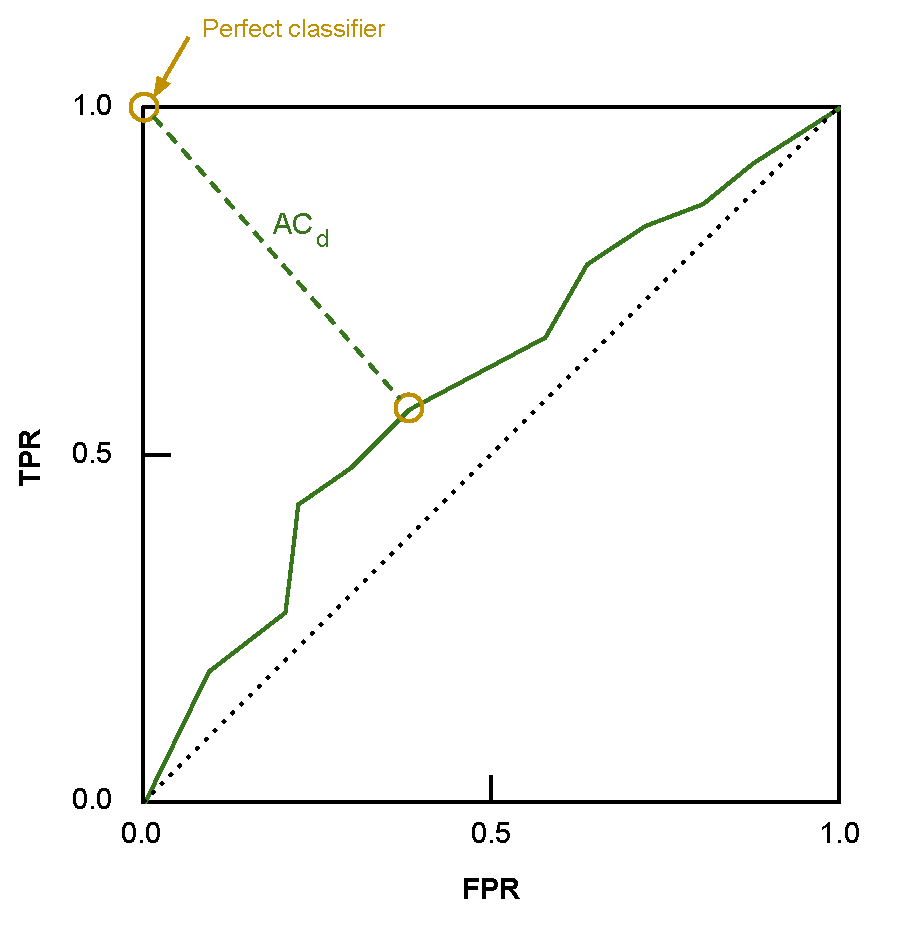
\includegraphics[scale=0.7]{images/roc.pdf}
\caption{ROC (receiving operator characteristics) curve. The $AC_d$ is the distance from a classifier's performance to that of a perfect classifier.}
\label{fig:roc}
\end{figure}

We still lack a single measure that could be used for ranking different classifiers. Since a perfect classifier is the point (0,1) on the ROC curve, we can rank the classifiers based on their distance to that point. Euclidean distance is defined as
\begin{equation}
\text{AC}_d = \sqrt{W \cdot (1 - \text{TPR})^2 + (1 - W) \cdot \text{FPR}^2}, \label{eq:acd}
\end{equation}
where the parameter $W \in [0,1]$ assigns relative importance to false positives and false negatives. The value of $\text{AC}_d$ ranges from 0 for a perfect classifier to $\sqrt{2}$ for a completely incorrect one. \cite{Hamilton12}

To summarize, the parameter selection process goes like this:
\begin{enumerate}
\item{Get parameters values one by one from the grid of available values}
\item{Calculate performance using cross validation and $\text{AC}_d$ as performance measure}
\item{Choose the parameters values with the best performance (highest accuracy or lowest $\text{AC}_d$)}
\end{enumerate}

\subsection{Computational Performance}
Computational performance is not one of the key concerns of this thesis but it is still worth reviewing the possible bottlenecks and ways to improve performance. Not only can the amount of data be huge in CEP, but also the latency with which it is moving should be minimal. That said, our system is of no use if it cannot keep up with new sensor data coming in.

At the core of our system is the Esper CEP Engine which, according to its documentation \cite{EsperReference}, can manage over 500,000 events per second on a dual-core CPU 2 GHz processor with engine latency being less than 3 microseconds on average. The processor on our own test machine is a quad-core CPU 2.5 GHz processor so the performance should be at least at the same level.

It is important to note that training the model does not need to be real-time. In a real-life application the model is trained with regular intervals as a background process. While a new model is being trained, the old model can continue predicting. When the new model is ready, the old model is replaced with it. For example, in our test house this could be done once a month when the indoor air conditions have changed because of, for instance, seasonal changes in the weather.

The prediction phase, in turn, has to be fast as new measurements are coming in all the time. With our DTW and kNN model the prediction includes calculating the DTW distance with each of the training vectors and then selecting \emph{k} closest ones. With our Wavelet and SVM model the prediction phase consists of the Haar Wavelet transform that produces a feature vector and support vector evaluation that classifies the feature vector.

Our computation performance tests evaluate the models' time complexity with respect to window sizes and the number of testing samples. Also the average execution times for classifying a single instance are measured.
